\chapter{Metodologia de Trabalho}
\label{chap:Metodo}

Neste capítulo é apresentado o método utilizado para o desenvolvimento deste trabalho. Foram envolvidos dois procedimentos de pesquisa científica e uma técnica de modelagem de design sobre as informações coletadas na pesquisa científica (Figura \ref{Fig:geral_flow.png}).

\begin{figure}[htbp]
	\centering
	\caption{Processo Metodológico do Trabalho}
	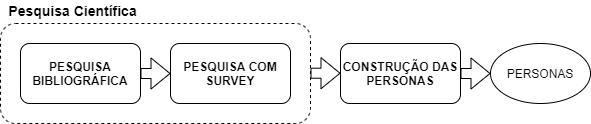
\includegraphics[keepaspectratio=true,scale=0.6]{figuras/metodologia/fluxo geral.png}
	\legend{Fonte: Autor}
	\label{Fig:geral_flow.png}
\end{figure}

As metodologias apresentadas na Figura \ref{Fig:geral_flow.png} seguem descritas nas seções a seguir. A Seção \ref{sec:pesq_cient} apresenta a metodologia de pesquisa bibliográfica e da pesquisa com \textit{survey} e a Seção \ref{sec:const_person} descreve o processo de construção das personas. 


\section{Pesquisa Científica} 
\label{sec:pesq_cient}

O primeiro passo do processo metodológico neste trabalho foi a realização de uma pesquisa científica (Figura \ref{Fig:geral_flow.png}). Segundo \citeonline[p. 34-42]{Gerhardt2009}, esta pequisa bibliográfica tem uma abordagem qualitativa, de natureza aplicada, com objetivo descritivo em relação aos conceitos sobre as personas, o método de criá-las e sobre as características de jogos para aprendizagem.

Nela foi realizada uma revisão da literatura não sistemática, na qual foram selecionadas trabalhos da literatura \cite{barbosa_silva, BarbosaEtAl2021, cooper07} recomendados pelos orientadores deste TCC. Também foi utilizada a literatura base do projeto de pesquisa Recursos Digitais Didáticos para Interação Humano-Computador\footnote{Repositório do projeto: \url{https://github.com/RecursosDigitaisdeEnsinoAprendizagemIHC}} (RDDIHC), artigos científicos publicados no projeto \cite{deSales_SousaeSilva_2020, silva_sales_mendes2021} e referências encontradas a partir da leitura destes. A interpretação e análise crítica das informações apresentadas na literatura adotada foram feitas pelo próprio autor deste trabalho \cite{ROTHER2007}. 

Na sequência foi realizado um \textit{survey}, como segundo passo do processo metodológico (Figura \ref{Fig:geral_flow.png}). Seu objetivo foi definir o perfil de usuários para jogos de aprendizagem em IHC, analisando suas preferências sobre algumas características e aspectos de qualidade em jogos, que foram identificadas na pesquisa bibliográfica, como os de \citeonline{Petri_Wangenheim_2019, deSales_SousaeSilva_2020}. Segundo \citeonline{Gerhardt2009}, a abordagem desta pesquisa é quali-quantitativo, de natureza aplicada, com objetivo descritivo utilizando-se de um questionário auto-aplicável para a realização da pesquisa com \textit{survey}. 

De acordo com \citeonline{Kasunic_2005} um \textit{survey} envolve a coleta e análise de dados na qual os entrevistados respondem a um instrumento de pesquisa previamente planejado. Um \textit{survey} consiste na execução de sete etapas, como apresentado na Figura \ref{Fig:survey_flow.png}.

\begin{figure}[htbp]
	\centering
	\caption{Processo de Pesquisa com Survey}
	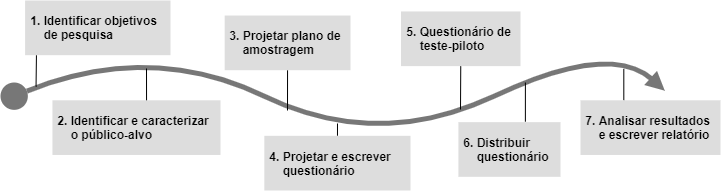
\includegraphics[keepaspectratio=true,scale=0.625]{figuras/metodologia/flow_survey.png}
	\legend{Fonte: Traduzido de \citeonline{Kasunic_2005}}
	\label{Fig:survey_flow.png}
\end{figure}

O processo se inicia com a identificação do objetivo de pesquisa como é apresentado na primeira etapa da Figura \ref{Fig:survey_flow.png}. O objetivo foi definido como ``identificar as características e aspectos de qualidade de jogos para aprendizagem, segundo o perfil dos usuários desse tipo de jogo''. Para se alcançar este objetivo foi necessário definir: quais os aspectos de qualidade dos jogos seriam analisados e quais características comporiam o perfil dos usuários de jogos para aprendizagem.

Seguindo o fluxo na Figura \ref{Fig:survey_flow.png}, na segunda etapa, identificação e caracterização do público-alvo, foi adotada como população os alunos de graduação e pós-graduação de cursos da área de Ciência da Computação. Esta população foi escolhida por conta da sua visão mais técnica quanto aos aspectos de qualidade de software, a familiaridade no uso de ferramentas digitais, além de serem os possíveis usuários de jogos digitais para aprendizagem.

A terceira etapa da Figura \ref{Fig:survey_flow.png} aborda a realização do plano de amostragem, que foi definido no presente trabalho para ser realizado em instituições de ensino de graduação e pós-graduação. A amostragem desta pesquisa é não probabilística, pois não é objetivo deste trabalho generalizar os resultados para fora do público-alvo \cite{Kasunic_2005}. Como pretende-se utilizar os resultados como uma proposta de uma ferramenta de design (as personas) de jogos para aprendizagem em cursos de computação não se faz necessário a generalização para fora da amostra.

A coleta dos dados foi planejada para ser executada via questionário virtual, no período entre os dias 06/10/2020 e 27/10/2020. O tamanho da amostra consistiu então nos registros de resposta coletados neste período. 

As perguntas elaboradas para o questionário (Apêndice \ref{ap:questionario}), na quarta etapa (Figura \ref{Fig:survey_flow.png}), buscaram identificar os atributos do modelo de personas apresentado por \citeonline{Courage_Baxter_2005}, apresentados na Subseção \ref{sub:def-pers}, além dos aspectos de qualidade de jogos para aprendizagem identificadas por \citeonline{deSales_SousaeSilva_2020} e as descritas por \citeonline{Petri_Wangenheim_2019}. A Tabela \ref{tab:Table_variaveis-quest} apresenta as variáveis relacionadas com as perguntas feitas no questionário do de pesquisa.

\begin{table}[htbp]
\centering
\caption{Variáveis do Questionário}
\label{tab:Table_variaveis-quest}
\begin{tabular}{|p{1.6cm}|p{9.5cm}|p{4cm}|}
\hline
\textbf{Questão} & \textbf{Variáveis}                         &  \textbf{Tipo }         \\ \hline
I01  & Idade                                      &  Identidade                         \\ \hline
I02 & Sexo                                       &  Identidade                             \\ \hline
I03  &  Nome da Instituição de Ensino              &  Identidade                               \\ \hline
I04 & Curso de Graduação em Ciência da Computação &  Identidade                             \\ \hline
O01   &  Relação com a Disciplina de IHC             & Identidade                               \\ \hline
H01   &  Experiência com design de interfaces        & Habilidades                               \\ \hline
RL01   &  Ação para sanar dúvidas de algum conteúdo   & Relacionamentos                         \\ \hline
O02  &  Uso de jogos para aprender                 & Objetivos                        \\ \hline
O02.1.1, O02.2.1, O02.3.1   &  Motivos para usar jogos para aprendizagem                 & Objetivos    \\ \hline
O02.1.2, O02.2.2   &  Frequência no uso de jogos para aprendizagem               & Tarefas              \\ \hline
O02.1.3, O02.2.3   &  Jogos para aprendizagem usados              & Tarefas             \\ \hline
O02.1.4  & Motivos para deixar de usar jogos para aprendizagem       & Objetivos                      \\ \hline
O02.3.2  &  Motivos de nunca ter usado jogos para aprendizagem        & Objetivos                     \\ \hline
O02.4.1  & Motivos de desinteresse em jogos para aprendizagem   & Objetivos                \\ \hline
RE01  & Relevância dos fatores de usabilidade do jogo             & Requisitos e Aspectos de Qualidade                        \\ \hline
E01   & Importância dos fatores de experiência do jogo            & Expectativas e Aspectos de Qualidade                          \\ \hline
\end{tabular}
\legend{Fonte: Autor}
\end{table}

A Tabela \ref{tab:Table_variaveis-quest} relaciona o identificador de uma questão do questionário de pesquisa (Tabela \ref{tab:quest-survey}), suas respectivas variáveis e o tipo da característica de persona definida por \citeonline{Courage_Baxter_2005}, citadas na Subseção \ref{sub:def-pers}. Estas são as variáveis definidas para compor o perfil dos jogadores. 

Já em relação aos aspectos de qualidade de jogos, são definidas as variáveis RE01 e E01 (Tabela \ref{tab:Table_variaveis-quest}). Estas variáveis representam os aspectos de qualidade de jogos, que juntamente analisadas com o perfil dos jogadores cumprem o objetivo do \textit{survey}.

O questionário passou por rodadas de teste, correções e melhorias, como prescreve a quinta etapa (Figura \ref{Fig:survey_flow.png}). Este teste contou com a participação de três pessoas. Foram coletados \textit{feedbacks} sobre a compreensão e o layout das perguntas, a estrutura e o fluxo do questionário, além de ser verificado o tempo médio para se concluir o questionário. O teste piloto foi realizado de forma virtual, via plataforma de vídeo-chamada.

Primeiramente o respondente recebeu algumas informações introdutórias sobre a pesquisa, em seguida ele acessou o questionário em seu computador e ativou o compartilhamento de tela. Dada a confirmação para o início da execução do questionário foram anotadas as percepções do avaliador enquanto o participante respondia.

Concluído o teste piloto foi solicitado um relato oral do responte sobre sua percepção ao longo da execução do questionário, as quais foram anotadas pelo avaliador. Este processo foi realizado com cada um dos três participantes do teste. Depois de analisadas as anotações, foram aplicadas as sugestões de melhoria e corrigidos os erros encontrados no questionário.

Na sequência, na sexta etapa (Figura \ref{Fig:survey_flow.png}), o questionário foi distribuído via mensagem eletrônica e redes sociais para as comunidades discentes: Universidade Católica de Salvador (UCSAL), Universidade de Brasília (UnB), Universidade Federal de Uberlândia (UFU), Universidade Federal do Amazonas (UFAM),  Universidade Federal do Mato Grosso (UFMT), Universidade Federal do Mato Grosso do Sul (UFMS) e Universidade Tecnológica Federal do Paraná (UTFPR). Durante o período estipulado para a pesquisa (quatro semanas), foi monitorada a quantidade de respostas obtidas, sendo que ao perceber uma baixa taxa de respostas nas duas primeiras semanas, foram enviadas novas mensagens ao público-alvo para que fosse reforçado a importância da participação deles na pesquisa.

Na última etapa, conforme a Figura \ref{Fig:survey_flow.png}, os dados coletados foram armazenados em uma planilha eletrônica e ali analisados. Foram obtidas 184 respostas, porém com inconsistências em algumas delas. Das inconsistências, 8 pessoas responderam o questionário mais de uma vez e 10 respondentes não cursaram graduação na área de computação. Essas dezoito respostas foram removidas, restando portanto, um total de 166 respostas válidas. 

Esta análise que se inicia na pesquisa com \textit{survey} e se estende para o processo de construção das personas. Na Seção \ref{sec:const_person} é apresentado este processo de análise e construção das personas.

\section{Construção das Personas}
\label{sec:const_person}

O processo de construção das personas descrito por \citeonline{cooper07} apresenta sete etapas para definir um elenco de personas. Neste trabalho estas etapas foram executadas em três fases. A Figura \ref{Fig:construct_persona.png} demonstra uma visão geral do processo.
\newpage

\begin{figure}[htbp]
	\centering
	\caption{Processo de Construção das personas}
	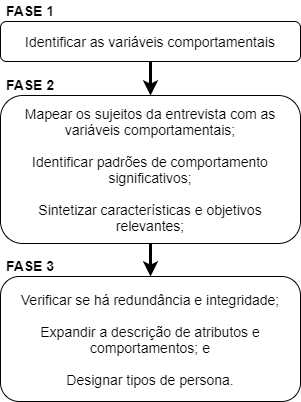
\includegraphics[keepaspectratio=true,scale=0.6]{figuras/metodologia/construct_persona.png}
	\legend{Fonte: Autor}
	\label{Fig:construct_persona.png}
\end{figure}


As respostas de cada indivíduo foram registradas na planilha eletrônica (PE0). Este conjunto de dados foi o ponto de partida para a modelagem das personas.

\subsection{Fase 1 da Construção de Personas}

Na primeira fase foram identificadas as variáveis comportamentais. Estas foram definidas a partir das variáveis do \textit{survey} (Tabela \ref{tab:Table_variaveis-quest}). Na Tabela \ref{tab:Table_variaveis-comp} estão as variáveis comportamentais identificadas. 

\begin{table}[htbp]
\centering
\caption{Variáveis Comportamentais}
\label{tab:Table_variaveis-comp}
\begin{tabular}{|p{4.7cm}|p{10cm}|}
\hline
\textbf{Questão} & \textbf{Variáveis}                             \\ \hline
O01   &  Relação com a Disciplina de IHC                          \\ \hline
H01   &  Experiência com design de interfaces                      \\ \hline
RL01   &  Ação para sanar dúvidas de algum conteúdo               \\ \hline
O02  &  Uso de jogos para aprender                \\ \hline
O02.1.1, O02.2.1, O02.3.1   &  Motivos para usar jogos para aprendizagem\\ \hline
O02.1.2, O02.2.2   &  Frequência no uso de jogos para aprendizagem\\ \hline
O02.1.4  & Motivos para deixar de usar jogos para aprendizagem       \\ \hline
O02.3.2  &  Motivos de nunca ter usado jogos para aprendizagem    \\ \hline
O02.4.1  & Motivos de não ter interesse em jogos para aprendizagem       \\ \hline
RE01  & Relevância dos fatores de usabilidade do jogo          \\ \hline
E01   & Importância dos fatores de experiência do jogo        \\ \hline
\end{tabular}
\legend{Fonte: Autor}
\end{table}

A Tabela \ref{tab:Table_variaveis-comp} relaciona o identificador de uma questão do questionário de pesquisa com suas respectivas variáveis. De acordo com as respostas dadas pelos respondentes, estes foram agrupados compondo grupos comportamentais com características semelhantes. A segunda fase de construção das pesonas detalha mais sobre este processo.  


\subsection{Fase 2 da Construção de Personas}
\label{sub:const-pers}
Após a identificação das variáveis comportamentais seguiu-se para segunda fase, como é apresentado na Figura \ref{Fig:construct_persona.png}. Os passos foram o mapeamento dos respondentes em relação a essas variáveis, a identificação de padrões de comportamento significativos e a sintetização de características e objetivos relevantes.

Fez-se uso da planilha eletrônica (PE0) e suas ferramentas para a auxiliar o processo de filtragem e síntese dos dados. Primeiramente foram divididos em dois, os dados dos respondentes, a partir da variável I04. Assim foi definida as primeiras características da anti-persona (aqueles que não são da área de Ciência da Computação) e a estrutura base das demais personas (PE1), aqueles que são da área da Ciência da Computação. Na Figura \ref{Fig:persona_tree.png} é apresentada o processo de refino dos dados para construção das personas.

\begin{figure}[htbp]
	\centering
	\caption{Fluxo do Processo de Construção das Personas}
	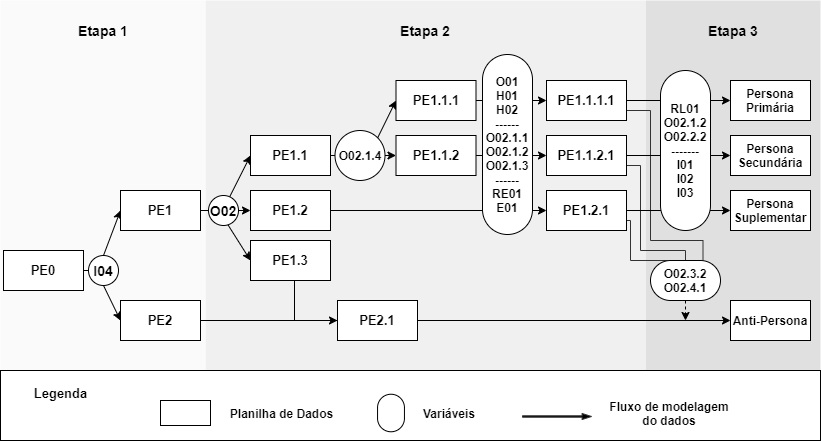
\includegraphics[keepaspectratio=true,scale=0.55]{figuras/metodologia/persona_tree.png}
	\legend{Fonte: Autor}
	\label{Fig:persona_tree.png}
\end{figure}


A partir da variável O02 foi possível agrupar os dados em três perfis comportamentais, a partir dos dados em PE1. Foram estes, o perfil daqueles que ainda usavam jogos e os que já usaram, mas não jogavam mais (PE1.1); o perfil  daqueles que nunca jogaram, mas tinham um interesse (PE1.2); e o perfil daqueles que não tinham interesse de jogar, que no caso foram englobado à anti-persona.

Dentro de PE1.1 existiam aqueles que já haviam jogado, mas por algum motivo tinham parado de usar jogos para aprendizagem. Destes, foram relevantes para o objetivo do trabalho apenas os que pararam de jogar por terem alcançado seu objetivo de estudo com estes jogos. Foi obtido então PE1.1.1, com  os dados daqueles que usavam jogos para aprendizagem e PE1.1.2, aqueles que haviam jogado, mas pararam por haverem alcançado seu objetivo de estudo, que no caso foram identificados pela variável O02.1.4. Já os que deixaram de jogar e não conseguiram alcançar seu objetivo de estudo com jogos, estes foram encorporados na anti-persona.

O próximo passo foi identificar, a partir das variáveis H01 e O01, quais os perfis comportamentais seriam mais frequentes para compor personas significativas. Nesta análise, os perfis comportamentais identificados expressavam que os respondentes tinha um conhecimento sobre design de interfaces, variando entre meios formais e não formais de educação. Enquanto que outros não tinham nenhum conhecimento, sendo que estes ou estavam fazendo o curso de IHC ou ainda não haviam feito.

Agrupados esses conjuntos de características foi possível definir os objetivos das personas (O02.1.1, O02.2.1 e O02.3.1). Foram os objetivos: busca por um jogo que auxiliasse no aprendizado de um conteúdo novo, um jogo que ajudasse na revisão de um conteúdo e um que fornecesse a possibilidade de avaliar o conhecimento do jogador, formando então os perfis PE1.2.1, PE1.1.1.1 e PE1.1.2.1. 

Com os objetivos das personas definidos, foram então determinadas os requisitos de jogos e as experiências (RE01 e E01, respectivamente) mais relevantes para cada um dos três perfis. Estes requisitos e experiências podem ser observadas no Apêndice \ref{ap:questionario}, nas Figuras \ref{tab:req-qualit} e \ref{tab:exp-player}, respectivamente.

Para definir a relevância de cada aspecto, foi utilizado o processo do trabalho de \citeonline{silva_sales_mendes2021} como base. A relevância de cada um destes aspectos de qualidade (requisitos do jogo e experiência do jogador) se deu pela classificação que os respondentes deram a cada aspecto: Não é importante; Pouco importante; Indiferente; Importante; e Muito importante (traduzidos numa pontuação de 0 a 4, respectivamente).

Cada um dos três perfis foi caracterizado por estes aspectos de qualidade, sendo que cada um deles obteve um grau de relevância entre 0 e 664. Este grau de relevância é reflexo do somatório da pontuação que todos os respondentes (166) deram para determinado aspecto. Esses limites (0 e 664) remetem ao caso, se todos os respondentes dessem a pontuação mínima (0) para um determinado aspecto, o grau de relevância seria 0, mas se todos dessem a pontuação máxima (4), o grau de relevância seria 644.

Supondo que fossem 5 respondentes e dois aspectos. Para o Aspecto 1 as pontuações de cada respondente respectivamente foram 3, 4, 2, 2 e 3, então o grau de relevância do Aspecto 1 seria de 12 pontos, dentro do intervalo de 0 a 20. Para o Aspecto 2 as pontuações de cada respondente respectivamente foram 4, 4, 1, 3 e 2, então o grau de relevância do Aspecto 1 seria de 14 pontos, dentro do intervalo de 0 a 20. Ou seja a persona que representa estes 5 respondentes teria o Aspecto 2 mais relevante que o Aspecto 1. 

\subsection{Fase 3 da Construção de Personas}

Com essa estrutura base das personas, foi realizada a terceira e última fase (Figura \ref{Fig:construct_persona.png}), que visa lapidar as personas. Foi verificada a integridade das personas e se existiam redundâncias entre elas. A descrição das personas foi então detalhada, inserindo mais atributos e comportamentos a partir das variáveis RL01, O02.1.2, O02.2.2, I01, I02 e I03. Estas serviram para dar mais realismo às personas e além disso cada persona recebeu uma foto que a representasse. 

Por fim, foram designados os tipos de personas: primária; secundária; e anti-persona. No caso da anti-persona, as variáveis O02.3.2 e O02.4.1 compuseram as características dela, além dos atributos considerados irrelevantes para as outras personas.

O elenco de personas construídas contemplou quatro personas, sendo elas: uma primária, duas secundárias e uma anti-persona. Este elenco assim como a análise e discussão sobre os resultados se encontram descritas nos Capítulos \ref{chap:result} e \ref{chap:ele-pers}.
